\begin{center}
   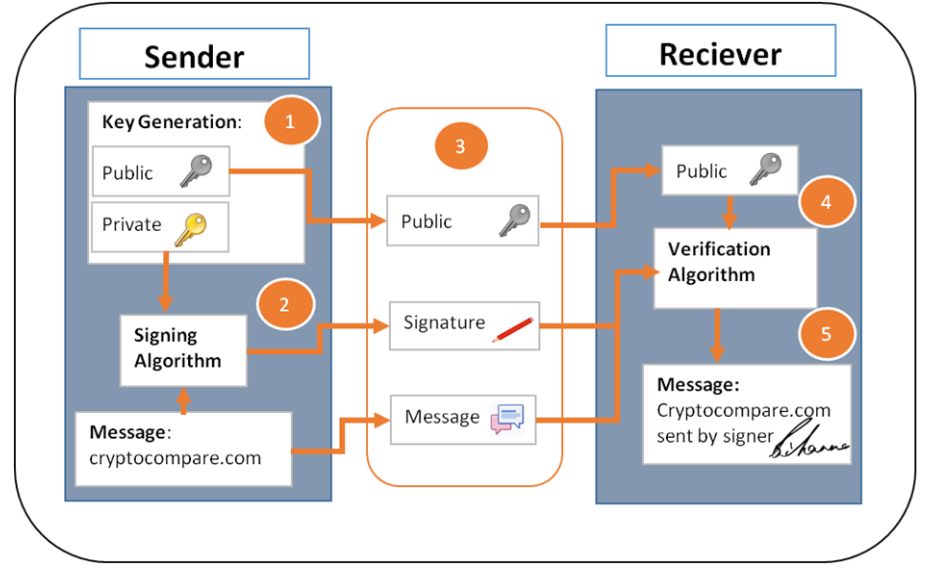
\includegraphics[scale = 0.35]{diagrams/transaction_diagram.png}
\end{center}

The diagram above shows how an operation (here a transaction on the bitcoin protocol) is carried out.

\begin{enumerate}
  
  \item You create a hash of the operation data (e.g. sender, receiver, message).
    Your private key is then used to sign this hash, to create a digital signature.

  \item You broadcast the operation data to the mining network, together with your digital signature and your public key.

  \item Now, mining nodes can compute inexpensively whether your public key and your digital
    signature where made using the same private key
    
  \item If the transaction is valid, it is added to the aforementioned pool of operations to be placed in a block.

  \item Mining race eventually ends and a block containing your operation is added to the chain.
    
\end{enumerate}
